
\documentclass[letterpaper]{article}



\usepackage{times}
\usepackage{uist}
\usepackage{graphicx}
\usepackage{url}
\newcommand{\remove}[1]{}

\begin{document}

% --- Copyright notice ---
\conferenceinfo{UIST'09}{October 4-7, 2009, Victoria, British Columbia, Canada}
\CopyrightYear{2009}
\crdata{978-1-60558-745-5/09/10}

% Uncomment the following line to hide the copyright notice
% \toappear{}
% ------------------------

\bibliographystyle{plain}

%\title{Standard UIST Conference Format:\\
%       Preparing Camera-Ready Submissions}
\title{Voicify: User Demonstrated Voice Interfaces}

%\author{Adam Vogel \and Arda Kara}

%%
%% Note on formatting authors at different institutions, as shown below:
%% Change width arg (currently 7cm) to parbox commands as needed to
%% accommodate widest lines, taking care not to overflow the 17.8cm line width.
%% Add or delete parboxes for additional authors at different institutions. 
%% If additional authors won't fit in one row, you can add a "\\"  at the
%% end of a parbox's closing "}" to have the next parbox start a new row.
%% Be sure NOT to put any blank lines between parbox commands!
%%

\author{
\parbox[t]{9cm}{\centering
	     { Adam Vogel}\\
     Computer Science Department\\
             Stanford University \\
	     av@cs.stanford.edu}
\parbox[t]{9cm}{\centering
	     { Arda Kara}\\
	     Computer Science Department\\
       Stanford University\\
	     ardakara@cs.stanford.edu}
}

\maketitle

\abstract
%Although voice interfaces exist for the main functions of modern mobile phones, many community-developed 
%applications lack speech support. 
We present \emph{Voicify}, a framework for voice programming by 
demonstration which enables users to build their own speech interfaces.
The user creates their own voice interface by demonstrating a voice command with the corresponding
actions to take on the phone. The phone can then be put in a hands-free mode, where it
responds to previously programmed voice commands. 
Transparency is a key issue, and we discuss the development of a voice-only keyboard for
text entry paired with a custom screen reader for giving feedback to the user.
We conducted a user study which shows that
interfaces created using Voicify rival their touch counterparts.
However, our study also shows that most users find programming by demonstration to be
tedious, and that the natural language processing is too impoverished to be widely applicable.

\section{Introduction}
Speech interfaces have been gaining in popularity with the proliferation of mobile devices. Smartphones are
frequently used in hands-free or eyes-free contexts, such as while driving or walking. Modern phones like
the iPhone and Android phones include speech recognition and synthesis in the operating system, allowing
users to make calls and send text messages by voice. However, there is a long tail of community authored
phone applications which have no voice interface. This is a big restriction for the convenience of
hands-free users and the sight disabled. 

To address this problem, we introduce \emph{Voicify}\footnote{The Voicify source code is available for download at \url{https://github.com/acvogel/astrid} and a demo video is available at \url{http://nlp.stanford.edu/acvogel/voicify.mov}.}, a framework for creating speech interfaces 
through end-user demonstration. Voicify allows a user to create voice commands for Android
applications through a ``tell and show'' interface: the user first \emph{tells} the phone what 
to do in natural language and then \emph{shows} the phone how to interpret this command.
Once the user has demonstrated commands, the phone can execute commands in a playback mode.

We further explore the efficacy of user demonstration and the usability of the resulting
interface by conducting a user study.  We \emph{voicified} a popular open-source Android to-do list
application called \emph{Astrid} \cite{astrid}. Using this version of Astrid, we tested the ease and
competence of the demonstration and playback interfaces when compared to the traditional touch
interface. Our results show that the voicified interfaces are usable, with a 60\% command interpretation
success rate, but still fall below the level needed for wide usage. Our user study revealed
several weaknesses in the demonstration interaction which we implemented.


The remainder of the paper summarizes the large body of work on programming by demonstration, details
the design and implementation of Voicify, and discusses the user study.





\section{Related Work}





Programming by demonstration has long been popular in the robotics community.
Early work includes the Robot Programming System (RPS) of SRI \cite{SRIpbd} and
Grossman \cite{grossman}, who taught robotic manipulators by manually controlling them.
More recent machine learning approaches to programming by demonstration 
go by the name \emph{apprenticeship learning}.
Abeel et al. \cite{Abbeel:2004:ALV:1015330.1015430} used human demonstrations of helicopter maneuvers to automatically learn difficult flying tricks. These approaches treat the demonstrator as an agent
acting in a reinforcement learning model and the system tries to infer the latent utility function
the agent is acting to maximize.

One of the difficulties of programming by demonstration is handling errors in 
the demonstration. Chen and Weld \cite{Chen:2008:RED:1378773.1378794} offer methods for
detecting inconsistent demonstrations, where the same command yields seemingly opposite
goals. They then use this detection to alert the user with disambiguating feedback.
Further, they use a probabilistic framework to measure the consistency of hypotheses,
treating uncertain parts of demonstrations as missing values.

Programming by demonstration has been studied in the user interface community as well.
Bocionek and Sassin \cite{Bocionek:1993:DLA:865219} improved room reservation systems
by observing the emails a receptionist received and the corresponding actions
he or she took to reserve a room. They specifically deal with the natural language problem,
and utilize a thesaurus to improve coverage.

In the natural language processing community there is an interest in learning to 
follow directions. Recent work which is applicable here is Branavan et al. 
\cite{DBLP:conf/acl/BranavanCZB09} who learned to interpret help guides for the 
Windows operating system. 
%Going back to the start of AI, McCarthy famously
%proposed an advice-taking robot \cite{McCarthy68programswith}, although in his approach
%the advice is encoded in logic, not natural language.

Lieberman \cite{lieberman2001} took programming by demonstration more literally, where users give examples
of what they would like to do and the computer attempts to generate code to 
achieve this goal. The user then interacts with the generated code, in the hopes
of making programming easier for beginners. In our case the user never 
modifies actual programming languages, but the principles involved are similar.

%TODO: \cite{Yankelovich:1995:DSI:223904.223952} speechacts paper.


\section{Programming by Demonstration}
The Voicify framework requires three main components: the ability to capture low-level UI events, 
an interface for recording demonstrations, and lastly the ability to playback commands for interpretation.

\subsection{UI Capture}
To record a command demonstration, Voicify requires access to the user interface actions that a user engages in.
Security restrictions on the Android platform make it impossible for a 3rd party application to capture 
touch and key events as this would enable malicious key loggers to steal sensitive information. 
The Android Accessibility Team \cite{androidaccessibility} confirmed that this is impossible to do without modifying the operating system.
To circumvent this problem, we chose an open-source application as a prototype, which allowed us to modify
the program source itself, thus capturing UI events within the application.

The UI design of Android still makes capturing UI events across a whole application a difficult task.
Within each screen, the interface elements, called \emph{views}, are arranged in a tree structure. When the user
touches the screen, the UI event is dispatched to the lowest element in the view tree which spans that portion of the 
screen. It is then passed up the view tree until a UI element consumes it. To capture these touch events,
we programmatically traverse the view tree and insert an invisible UI layer at each node. The UI layer
simply captures the UI interactions which pass through it.

Furthermore, some UI widgets like buttons and dialog boxes consume touch events without passing them along
to the activity in which they reside. Complicating matters, these boxes are required to be leaves
of the view tree, which doesn't allow for our trick of inserting invisible layers. To deal with these issues
we overrode the UI widget classes to capture the interactions. This required changing the UI definitions for
each of the screens to use our modified versions. This challenges our goal of making Voicify applicable to
every application but is a necessary hack for this prototype.

Lastly, each screen in an Android application is run in its own process, which pauses when switching between
screens in an application. This makes it difficult to share UI events across activities, which naturally
happens when demonstrating some commands. To overcome this we implemented a \emph{demonstration service} which runs in the background
of the application and aggregates UI interactions across activities.

When recording UI events, we capture low-level touches. The information in touch events includes the (X,Y) coordinate
on the screen, the pressure and size, and lastly whether it is initial contact, a dragging motion, or a release.
Our various capturing shims transmit these events to the demonstration service, which associates them with the
correct command. 

\begin{figure}[t]
\begin{center}
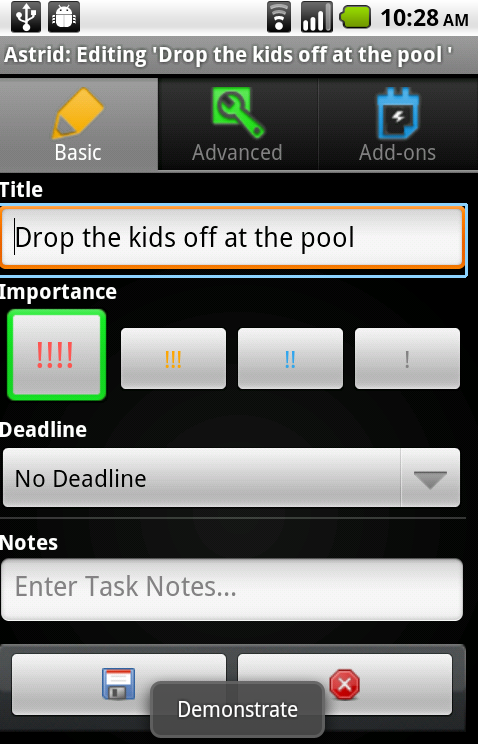
\includegraphics[scale=0.3]{fig/screenshot-cropped.png}
\end{center}
\caption{When the user presses the camera button a small UI notification appears to let them know to being demonstration.}
\label{fig:interface}
\end{figure}

\remove{Recording demonstrations at this low-level is the source of some errors. For instance, imagine
the user demonstrates how to click the 'save' button on a screen with a list. If the user later adds elements to the
list and tries to play back the 'save' command, the button might have moved. This is a large source of error in 
our experiments.}


%TODO: figure for the demonstration service? like boxes and arrows and shit.

\subsection{Demonstration Interface}
We now describe the user demonstration interface. We modified the hard camera button on the phone to serve as the 
``Voicify button''. After loading the Astrid application, the user presses the camera button. This pops up a small
notification which says ``Demonstration'' (see Figure \ref{fig:interface}). From here the user says the command that they would like to record,
for instance ``create a new task''.
After running Google-powered speech recognition, the interface speaks back to the user what it thinks the command
is, such as ``recording command 'create a new task' ''. The phone now is in capture mode, where all subsequent
UI events are associated with this command. After executing the desired sequence of interactions, the user
again presses the camera button to signal the end of demonstration, which triggers a small pop-up window
to acknowledge the demonstration.

We use the hard camera-button to solve the \emph{clutching problem}, which is how to determine when a trial has ended.
We also experimented with a soft button in a context menu within the application, but users found it cumbersome
to locate, whereas the hard camera button is able to be pressed by feeling alone.
A better demonstration interface would be to always capture the audio and only record when the 
user says a key phrase. However, the current state of speech recognition is not good enough to enable this.




\subsection{Playback Interface}
The Android operating system employs a sandbox-based security framework that prevents any interaction between applications. 
Each application has its own virtual machine, which makes it more difficult to implement a system-wide voice control interface without modifying the OS.
Our workaround was to use the UI testing features of the built-in unit testing tools that come with the Android SDK.
One downside of this approach is that the phone needs to be plugged into the debugging environment during testing; however, 
this didn't come up as a concern from our test users. Listening for the commands was still done on the phone, 
and the Astrid application was modified to receive a voice command upon a button press, look-up the closest matching voice command 
that it has in its database, and send the necessary UI interactions to the test suite using IPC. Our system for receiving commands used 
a word overlap index to find the closest command in its database. Just like the demonstration interface, the user would press a button 
and then utter the voice command they want to use. The phone then echoes the command that it thinks it received and carries out the 
recorded UI interactions. 
 

When using Voicify in an eyes-free environment, the application needs to read information the user in addition to interpreting commands.
Android has a built-in screen reader tool called TalkBack that can be turned on as a system-wide setting and allows the user to get 
voice feedback from their interactions by traversing through UI elements using the d-pad on their phones (if available on the model). 
%An alternative to TalkBack is a third-party open source tool called Spiel that allows per-application customization through JavaScript. 
Our system did not use TalkBack, as it required the phone's accessibility mode to be turned on which intervened with 
custom accessibility objects that our code uses. Instead, we implemented a replacement that dispatches d-pad commands to traverse 
through visible UI elements, and simulates accessibility events to gather readable content at each step. This worked well for a uniform 
screen like the list of to-do tasks, but got in the way of user interaction in more complicated screens due to the simulated traversal. 
Therefore we only used the screen reader to read off the list of tasks.

We also wanted the voicified interface to be able to accept new input for text fields. For 
example, if the user demonstrated a voice command for creating a new to-do task, the title for the task should be customizable during
playback. To achieve this, we implemented a voice keyboard for Android that is available across applications. 
Once the voice keyboard is selected as the system-wide keyboard, the phone asks you to speak anytime a field that needs the keyboard is selected. 
This meant that any demonstration that ends with a text input field selected would know to prompt the user to speak again after 
the voice command and enter the transcribed text into the text field. Obviously, a limitation of this is that it did not allow 
demonstrations to accept input in between touch commands. Any demonstration that accepts input needed to do so as the very last step, which
some users found confusing.

%The text-to-speech and speech-to-text engines that we used are made available in Android by Google. The speech-to-text transcriber 
%is a network solution that sends the voice command files to Google's servers and returns the best transcription guess for the 
%audio. This system often gave very accurate results on one of our phones and did not perform as well on the other. It is worth noting 
%that the phone with worse speech recognition might have introduced a lower than expected task completion success rate.  



\section{Method}

\begin{figure}[t]
\begin{center}
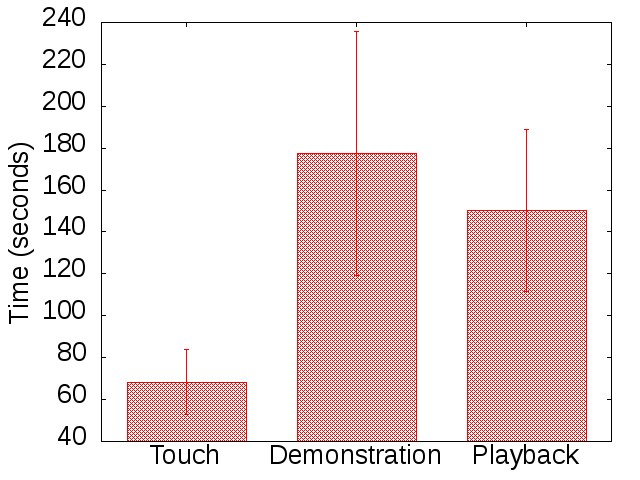
\includegraphics[scale=0.4]{fig/results.jpg}
\end{center}
\caption{The amount of time each of the seven tasks took for each user interface. The speech interfaces are significantly slower than the touch interface.}
\label{fig:results}
\end{figure}

We conducted a lab user study two questions:
\begin{enumerate}
\item Do users find our demonstration interface natural to use?
\item Are voice interfaces created by demonstration capable of achieving the same features as touch interfaces?
\end{enumerate}

To do so, we recruited 10 members of Stanford University to participate in a user study. We focused on a representative set of 
seven tasks in the Astrid to-do app:
\begin{enumerate}
\item Create a new task
\item Add a title
\item Set the task priority to high
\item Add a note
\item Toggle the reminder
\item Delete a task
\item Save a task
\end{enumerate}
The participants began by experimenting with the Astrid application for a few minutes to familiarize themselves with its layout.
From here the participants were given the list of commands, written out in the above form, and asked to complete them using
the touch interface. This served two purposes: to provide a baseline of the amount of time the tasks take, and to further
familiarize the users with the parts of the interface they will be demonstrating. Here we recorded the UI interactions
of the user to verify task completeness and recorded the amount of time it took.

Next the experimenters explained the demonstration interface and programmed a sample command to show the user how it works.
The users were then instructed to program voice commands to complete the tasks. The printed instructions were
still available to users, but surprisingly few directly read the printed instructions. When speech recognition errors
occurred, some users re-recorded the command, and others simply moved on. The quality of speech recognition and demonstration
in this phase is critical for creating a good interface. However, not all errors are fatal. Sometimes the transcription
errors are systematic, meaning that if the user says the same thing at playback the command will still work, despite
the fact that the speech is misinterpreted.

After completing the demonstration phase, the phone was put into playback mode by starting the UI test environment
on the connected laptop. The users then did the seven tasks once again, and the success of each completing
each step was recorded. Users were instructed that if they could not complete a task after several attempts
to continue to the next one.

%To test the efficacy of Voicify, we ran a study with 10 subjects. They were first asked to 
%familiarize themselves with the phone and the Astrid application. They, then, were given a list of tasks to carry out and 
%asked to first do them by using the conventional touch interface, then record voice commands for these tasks using our 
%demonstration interface, and finally carry out the tasks using the resulting voice interface. The list included actions that are typically 
%carried out in a to-do application, such as creating a task, editing the title and the importance of the task, adding notes, and checking 
%off items from the list. We measured the time it takes the subjects to complete the list 
%using each interface, and their task completion success rates using the Voicify interface. 



\section{Results}

Figure \ref{fig:results} shows the amount of time users spent in each mode. As expected, users completed the tasks in less time using the touch interface.
The demonstration period took the longest, as users had to both state their actions and execute them in the UI. Playback took slightly less time due to the
phone automatically executing touch actions. We found a relatively wide range of the time spent by participants. This can be attributed to systematic
differences in speech recognition quality across users.

In playback mode, users successfully completed tasks 58.6\% of the time, with a standard deviation of 23.6\%. This is a relatively high variation across
users. Several users were able to complete all but one of the tasks successfully, and several completed almost none. 

\subsection{Discussion}
Errors in playback mode can be
grouped into several classes:
\begin{itemize}
\item Speech recognition errors. Sometimes the system mis-interprets the command given.
\item Demonstration mistakes. Some users incorrectly demonstrated how to carry out commands.
\item Cascading errors. When the system makes errors on parts of a larger task, the user can become uncertain of the state of the application, causing command to be played incorrectly.
\end{itemize}
The errors in speech recognition are difficult to deal with. By echoing the user command both at demonstration and playback time we hoped to provide \emph{transparency} to the user.
However, even if users are aware that the system makes an interpretation error, it can be difficult to recover from without appropriate commands. Some users found that the
interface was overly verbose - listening to the system read back commands can be tedious. Possible approaches to this problem follow trends in normal dialog-systems, which frequently
use the confidence of speech recognition to decide when to ground user commands \cite{DBLP:journals/csl/YoungGKMSTY10}.

Other errors were caused by the brittleness of our demonstration representation. Low-level touch
events are highly context sensitive and do not generalize across interfaces. For instance,
correctly pressing the `save' button on one screen can differ from another. Furthermore, we did
not represent the screen on which a command was demonstrated, thus it sometimes executes  commands which 
are not applicable to a given UI state. A first step in this direction would be to represent the 
specific UI element that was manipulated instead of just recording $(x,y)$ coordinates. We could 
further leverage cues like the labels on buttons or dialog boxes to aid command interpretation,
similar to \cite{DBLP:conf/acl/BranavanCZB09}.



\section{Conclusion}
We presented \emph{Voicify}, a demonstration framework for mobile Android applications.
Our user study provided several key insights into successful programming by demonstration.
Users require an abstract representation of instructions, above the UI level. Demonstrations
should take into account program context and the overall goals of the user.
Our study showed that speech recognition quality is critical to good performance, but that
existing technology is almost good enough.
Despite the fact that the speech interfaces learned through demonstration are not yet at the
level of their traditional touch counterparts, this work shows a promising route
towards providing wide-coverage voice interfaces to mobile applications which currently lack them.

\bibliography{voicify}

\end{document}
